\providecommand{\pdfxopts}{a-1b,cyrxmp}
\providecommand{\thisyear}{2022}
\immediate\write18{rm \jobname.xmpdata}%  uncomment for Unix-based systems
\begin{filecontents*}{\jobname.xmpdata}
        \Title{Проект рабочей программы дисциплины "Цифровая электроника" \textemdash\thisyear}
\Author{Артем Николаевич Прокшин}
\Creator{pdfTeX + pdfx.sty with options \pdfxopts }
\Subject{Проект рабочей программы дисциплины "Цифровая электроника"}
\Keywords{цифровая и микропроцессорная техника, ковариантные и контравариантные координаты, MexBIOS Development Studio, электрические машины}
\CoverDisplayDate{март \thisyear}
\CoverDate{2022-05-16}
\Copyrighted{True}
\Copyright{Public Domain}
\CopyrightURL{http://github.com/trot-t}
\Creator{pdfTeX + pdfx.sty with options \pdfxopts }
\end{filecontents*}


%\documentclass[a4paper,14pt]{article}
\documentclass[a4paper,14pt]{article}

\pdfcompresslevel=9

\usepackage[\pdfxopts]{pdfx}[2016/03/09]
\PassOptionsToPackage{obeyspaces}{url}
\let\tldocrussian=1  % for live4ht.cfg

%\usepackage{lscape}
%%% Страница
\usepackage[english,russian]{babel}
\usepackage{extsizes} % Возможность сделать 14-й шрифт
\usepackage{geometry} % Простой способ задавать поля
        \geometry{top=25mm}
        \geometry{bottom=30mm}
        \geometry{left=30mm}
        \geometry{right=30mm}
 %

\usepackage[T1,T2A]{fontenc}
\usepackage[utf8]{inputenc}
\usepackage{amssymb,amsmath}
\usepackage{float}
\usepackage[unicode, pdftex]{hyperref}
\usepackage[europeanresistors,americaninductors]{circuitikz}
\usetikzlibrary{calc}
\usepackage[T1,T2A]{fontenc}
\usepackage[utf8]{inputenc}

\usepackage{amssymb,amsmath}
\usepackage{float}
\usepackage[unicode, pdftex]{hyperref}
\usepackage{csquotes}

\usepackage{tikz}
\usepackage{rotating}
%\usepackage[landscape]{geometry}
\usepackage{graphicx}
\graphicspath{{pictures/}}
\DeclareGraphicsExtensions{.pdf,.png,.jpg}
\usepackage{pgfplots}
\usepackage{wrapfig}
\usepackage{rotating}
\usepackage{lipsum}
\usepackage{nccmath}
\usepackage{caption}
\usepackage{siunitx}
%\usepackage[american,cuteinductors,smartlabels]{circuitikz}
%\usepackage[backend=biber]{biblatex}

\usepackage[]{hyperref}
\ctikzset{bipoles/thickness=1}
\ctikzset{bipoles/length=0.8cm}
\ctikzset{bipoles/diode/height=.375}
\ctikzset{bipoles/diode/width=.3}
\ctikzset{tripoles/thyristor/height=.8}
%\ctikzset{tripoles/thyristor/width=1}
\ctikzset{tripoles/thyristor/width=0.8}
\ctikzset{bipoles/vsourceam/height/.initial=.7}
\ctikzset{bipoles/vsourceam/width/.initial=.7}
\tikzstyle{every node}=[font=\small]
\tikzstyle{every path}=[line width=0.8pt,line cap=round,line join=round]

\ctikzset{resistor = european}
\ctikzset{inductor = american}
\ctikzset{tripoles/thyristor/height=0.55}

\ctikzset{bipoles/cuteindictor/coils/.initial=3}
\ctikzset{bipoles/americanindictor/coils/.initial=3}
\ctikzset{bipoles/cuteindictor/coils/.initial=3}
\ctikzset{bipoles/americanindictor/coils/.initial=3}
\hypersetup{
colorlinks=false,
}
\usepackage{textcomp}

\graphicspath{{images/}}

\begin{document}

\pagenumbering{gobble} 

%\hfill\begin{tabular}{@{}p{.5\linewidth}@{}}
%\multicolumn{1}{@{}c@{}}{Some title} \\
%\lipsum[4]
%\end{tabular}

%\begin{tabular}{@{}p{.6\linewidth}@{}}
%\multicolumn{1}{@{}c@{}}{} \\
%\begin{minipage}{11cm}
%УТВЕРЖДАЮ
%
%Директор департамента образования
%
%\_\_\_\_\_\_\_\_\_\_\_\_\_\_\_\_\_ М.С. Куприянов
%
%«\_\_\_\_»\_\_\_\_\_\_\_\_\_\_ 2022 г.
%
%\end{minipage}\\
%\end{tabular}

\vspace{5cm}

\begin{center}
ПРОЕКТ РАБОЧЕЙ ПРОГРАММЫ

дисциплины

\emph{«ЦИФРОВАЯ ЭЛЕКТРОНИКА»}

для подготовки бакалавров

по направлению

13.03.02 «Электроэнергетика и электротехника»

по профилю

«Электропривод и автоматика»

\vspace{5cm}
старший преподаватель Прокшин А.Н.

\vspace{0.4cm}

кафедра РАПС

\vspace{0.4cm}

Санкт-Петербургский государственный электротехнический университет «ЛЭТИ» им. В.И. Ульянова (Ленина)

\vspace{8cm}

\textbf{Санкт-Петербург}

\textbf{2022}
\end{center}

%\begin{section}{ЛИСТ СОГЛАСОВАНИЯ}

%Разработчики:
%\\

%\noindent старший преподаватель Прокшин А.Н.

%\end{section}
\newpage

\begin{section}{СТРУКТУРА ДИСЦИПЛИНЫ}

\begin{tabular}{ll}
Обеспечивающий факультет & ФЭ \\
Обеспечивающая кафедра   & РАПС\\
Общая трудоемкость (ЗЕТ) & 3 \\
Курс                     & 3 \\
Семестр                  & 5 \\
\bf{Виды занятий} \\
Лекции (академ. часов)   & 34 \\
Лабораторные занятия (академ. часов) \\
Практические занятия (академ. часов) & 17 \\
Иная контактная работа (академ. часов) & 1\\
Все контактные часы (академ. часов) & 52 \\
Самостоятельная работа, включая часы на контроль
(академ. часов) & 56 \\
Всего (академ. часов) & 108\\
\bf{Вид промежуточной аттестации}\\

Зачет с оценкой (курс) & 3 \\
Курсовая работа (курс) \\
 
\end{tabular}

\end{section}

\newpage

\begin{section}{АННОТАЦИЯ ДИСЦИПЛИНЫ \\ «ЦИФРОВАЯ ЭЛЕКТРОНИКА»}

Изучаются архитектура современных цифровых систем управления с микроконтроллерами, основные этапы анализа, синтеза и проектирования таких систем. Подробно рассматриваются вопросы математического описания систем управления с микроконтроллерами, анализ и синтез с использованием методов как классической, так и современной теории управления. Теоретическая часть курса сопровождается практическими и лабораторными занятиями для практического освоения изученного материала.

\end{section}

\newpage
\begin{section}{Актуальность}
\begin{itemize}
\item \colorbox{yellow}{\parbox[t]{\textwidth}{упрощение системы управления с использованием
ковариантных (измеряемых) и контравариантных
(неизмеряемых) координат;}}
\item создание мобильных лабораторных стендов;
\item использование российского программного обеспечения;
\item использование российских микроконтроллеров в части задач
\end{itemize}
\end{section}

\newpage
\begin{section}{Компетенции}
{\bf ОПК-2} Способен применять соответствующий физико-математический аппарат, методы анализа и моделирования, теоретического и экспериментального исследования при решении профессиональных задач

\subsection*{Знать}
\begin{itemize}
\item геометрические основы измерения трехфазного тока
\item 
\colorbox{yellow}{\parbox[t]{\textwidth}{среды разработки и моделирования встроенного программного обеспечения систем управления электродвигателями, технологическими комплексами}}
\end{itemize}
\subsection*{Уметь}
\begin{itemize}
\item
\colorbox{yellow}{\parbox[t]{\textwidth}{применить среды разработки и моделирования MexBios Development Studio, SimInTech, Texas Instrument CCS, Motor Control Workbench, GCC toolchain для создания программы управления инвертором электрическими машинами}}
\end{itemize}
\subsection*{Владеть}
\begin{itemize}
\item
\colorbox{yellow}{\parbox[t]{\textwidth}{настройкой взаимодействия сред разработки с микроконтроллером и конечным оборудованием, отладка, поиск и устранение неисправностей в программе}}
\end{itemize}
\end{section}

\newpage
\section{Используемые в обучении информационные и \enquote{сквозные} технологии, цифровые инструменты}
\begin{itemize}
\item\colorbox{yellow}{Современные проблемы инфраструктуры электродвижения} \href{https://www.np-sr.ru/}{\enquote{НП Совет рынка}}, \href{https://www.atsenergo.ru}{АО \enquote{АТС}}, криптография ГОСТ, PKI, ocsp, проверка электронных подписей
\item\colorbox{yellow}{11 тем связанных с изображающими векторами} Современная геометрия, ковариантные и контравариантные координаты векторов, двойственные дуальные базисы, \url{overleaf.com}, \url{geogebra.com}, \url{www.latex4technics.com}, \url{https://www.tflex.com}.
\item\colorbox{yellow}{Преобразование базисов и координат из одной системы в другую} Матричный анализ, \href{http://www.reduce-algebra.com/}{reduce-algebra}, \href{https://maxima.sourceforge.io/ru/}{maxima}, \url{overleaf.com}, \url{geogebra.com}, \url{www.latex4technics.com}, \url{https://www.tflex.com}.
\item\colorbox{yellow}{Интегрированные системы программирования микроконтроллеров} \href{https://mechatronica-pro.com/ru}{MexBIOS}, \href{http://motorcontrol.ru}{среда НПФ Вектор}, \href{ti.com}{CodeComposerStudio}, \href{st.com}{STM32CubeIDE}, arm-none-eabi-* toolchain, st-link, DFU

\item\colorbox{yellow}{Принципы работы одно- и трех-фазного мостового инвертора напряжения} Моделирование работы инвертора
\href{http://www.raps-lab.eltech.ru/cgi-bin/circuit.pl}{на сервисе кафедры РАПС},
\href{http://www.geda-project.org/}{geda}, \href{http://ngspice.sourceforge.net/}{ngspice}, \href{easygeda.com}{easyEDA}, \href{https://simintech.ru/}{SimInTech}
\item\colorbox{yellow}{Отладка программ и блоков в МехBIOS, SimInTech и в облачных сервисах} \href{https://www.mycompiler.io/new/c}{песочница C},
\href{http://cpp.sh/}{песочница С++}, gcc, \url{overleaf.com}
\item\colorbox{yellow}{Отчеты оформляются исключительно по ЕСКД}  latex, \url{overleaf.com}
\item\colorbox{yellow}{Исходные коды блоков, шаблоны заданий и отчетов располагаются в системе контроля версий git с настроенной связью в overleaf и C-песочницами} \href{https://git-scm.com}{Git}, \href{https://github.com/trot-t}{github.com}, \href{https://www.mycompiler.io/new/c}{песочница C}, \url{overleaf.com}
\end{itemize}

\newpage
\section{Лекционный блок}
\begin{itemize}
\item[\bf{Тема 1}]{Современные проблемы инфраструктуры электродвижения}
      \begin{itemize}
          \item недостаточная мощность и кол-во зарядных станций (преобразователей электрической энергии) для электрических автомобилей, судов
          \item логистика и планирование заряда/разряда батарей автономного электрического транспорта
          \item \colorbox{yellow}{транспондеры, смартконтракты, российская криптография, блокчейн}
       \end{itemize}
\item[\bf{Тема 2}]{Передача активной и реактивной мощности между электрической машиной и промышленной сетью}
      \begin{itemize}
        \item изображающие векторы напряжения и тока
        \item реактивная мощность стекает с повышенного напряжения
        \item вектор напряжения передающей активную мощность электрической машины обгоняет вектор приемника
        \item вектор тока одинаков для обеих машин
      \end{itemize}
\item[\bf{Тема 3}]{Принципы работы однофазного мостового инвертора напряжения}
     \begin{itemize}
        \item   чисто активная нагрузка,
        \item нагрузка или источник содержит индуктивность или дроссель,
        \item работа обратного диода,
        \item передаваемая мощность при медленно меняющемся токе и быстро меняющемся напряжении в зависимости от скважности
      \end{itemize}
\item[\bf{Тема 4}]{Принципы работы трехфазного мостового инвертора напряжения}
  \begin{itemize}
   \item порядок переключения ключей,
   \item график токов в фазах при активной нагрузке,
   \item графики фазных и линейных напряжений,
   \item изображающие вектора фазных и линейных напряжений и токов
  \end{itemize}
\item[\bf{Тема 5}]{Работа ключей при векторной широтно-импульсной модуляции в трехфазном мостовом инверторе напряжения}
  \begin{itemize}
   \item таблица векторов состояний,
   \item нулевой вектор состоит из 2-х состояний,
   \item изображающий вектор как центр тяжести состояний взвешенных по времени нахождения в данном состоянии,
   \item потенциалы фаз и нуля
  \end{itemize}
\item[\bf{Тема 6}]{Синусоидальная широтно-импульсная модуляция в однофазном или трехфазном мостовом инверторе напряжения}
   \begin{itemize}
    \item наличие реального или \enquote{виртуального} нулевого провода,
    \item отличие активной мощности при синусоидальной и векторной широтно-импульсной модуляциях
  \end{itemize}
\item[\bf{Тема 7}]{Системы координат. Преобразование базисов и координат из одной системы в другую}
  \begin{itemize}
   \item разложение вектора по координатным осям по правилу параллелограмма,
   \item матрица преобразования
 \end{itemize}
\item[\bf{Тема 8}]{Системы координат в современной геометрии, косоугольная система координат, ковариантные и контравариантные координаты в косоугольной системе координат}
  \begin{itemize}
   \item \colorbox{yellow}{\parbox[t]{0.9\textwidth}{формула длины вектора в косоугольной системе координат $|\vec{x}|=\sqrt{x_1x^1 + x_2x^2}$,}}
   \item \colorbox{yellow}{\parbox[t]{0.85\textwidth}{скалярное произведение двух векторов $\vec{x}\cdot\vec{y} = x_iy^i =  x^iy_i$,}}
   \item \colorbox{yellow}{правило Эйнштейна},
   \item сравнение с прямоугольной декартовой системой координат
  \end{itemize}
\item[\bf{Тема 9}]{Измеряемые мгновенные значения токов и напряжений и их связь с ковариантными координатами}
  \begin{itemize}
   \item преобразование Блонделя $\vec{i} = \frac{2}{3}\left(i_a \vec{e}_a + i_b \vec{e}_b + i_c \vec{e}_c\right)$,
   \item \colorbox{yellow}{\parbox[t]{\textwidth}{формула для $\vec{i}$ в симметричной системе координат, полусумма контравариантых координат равна контравариантной координате
         $$
             i_a = \frac{1}{2}\left(i^a_\text {в осях AB} + i^a_\text{ в осях AC} \right)
         $$}}
  \end{itemize}
\item[\bf{Тема 10}]{Управление ШИМ через центр тяжести весов векторов состояния инвертора и связь с контравариантными координатами}
   \begin{itemize}
   \item \colorbox{yellow}{\parbox[t]{\textwidth}{правило рычага Архимеда для определения цента тяжести весов векторов состояния инвертора}},
   \item \colorbox{yellow}{\parbox[t]{\textwidth}{матрица преобразования ковариантных (измеренных) координат к контравариантным (координатам управления) изображающего вектора напряжения}}
  \end{itemize}
\item[\bf{Тема 11}]{Активная мощность, скалярное произведение в косоугольной системе координат}
  \begin{itemize}
   \item физическая величина есть сумма произведений ковариантной и контравариантной координат $i_k\cdot u^k$,
   \item поднимание и опускание индексов $i_k\cdot u^k = i^k\cdot u_k$,
   \item линейное напряжение как контравариантная координата в осях фазного тока,
   \item \colorbox{yellow}{\parbox[t]{\textwidth}{формула мощности в трехфазной сети через ковариантные и контравариантные координаты}}
  \end{itemize}
\item[\bf{Тема 12}]{Реактивная мощность в координатах косоугольной системы}
  \begin{itemize}
  \item связь реактивной мощности с векторным произведением
  \end{itemize}
\item[\bf{Тема 13}]{Напряжение индукции в координатах косоугольной системы}
  \begin{itemize}
  \item при неизменном амплитудном значении тока напряжение индукции перпендикулярно вектору тока,
  \item \colorbox{yellow}{\parbox[t]{0.85\textwidth}{перпендикуляр к вектору через двойственные координаты \\ $(I_A, I_B)\cdot (-I^B, I^A)$, где $I^i$ в двойственном базисе}}
  \end{itemize}
\item[\bf{Тема 14}]{Генерация широтно-импульсной модуляции с помощью таймера, варианты пилообразных сигналов, определение скважностей $T_A$, $T_B$, $T_C$}
  \begin{itemize}
  \item {принцип работы таймера, период, время срабатывания таймера},
   \item виды пилы таймеров,
   \item запись и извлечение уставок таймера в теневой (shadow) регистра,
   \item {формула перевода весов состояний в уставки таймеров $T_A$, $T_B$, $T_C$}
  \end{itemize}
\item[\bf{Тема 15}]{Использование неопределенности скважностей $T_A$, $T_B$, $T_C$ для уменьшения нагрева силовых ключей}
  \begin{itemize}
   \item мощность потерь силовых ключей,
   \item спектральный состав
  \end{itemize}
\item[\bf{Тема 16}]{Аналогово-цифровое преобразование}
  \begin{itemize}
   \item принцип работы АЦП,
   \item зависимость точности АЦП от времени оцифровки,
   \item запуск АЦП от прерывания ШИМ
  \end{itemize}
\item[\bf{Тема 17}]{Интегрированные системы программирования микроконтроллеров}
   \begin{itemize}
    \item \colorbox{yellow}{\parbox[t]{0.8\textwidth}{российские системы MexBIOS, VectorIDE, SimInTech}}
    \item {зарубежные системы фирм Texas Instrument, STM, Infineon}
   \end{itemize}
\item[\bf{Тема 18}]{Построение систем управления в МехBIOS}
  \begin{itemize}
   \item распределение памяти в микроконтроллере,
   \item драйверы GPIO,
   \item драйверы АЦП,
   \item драйверы ШИМ,
   \item драйверы SPI,
   \item осциллограф,
   \item блоки управления
  \end{itemize}
\item[\bf{Тема 19}]{Написание пользовательских блоков в системе MexBIOS}
       \begin{itemize}
          \item переменные портов ввода-вывода
          \item внутренние переменные
          \item компиляция блоков, библиотек, ядра системы
       \end{itemize}
\item[\bf{Тема 20}]{Отладка программ и блоков в МехBIOS}
      \begin{itemize}
        \item \colorbox{yellow}{\parbox[t]{0.8\textwidth}{отладка алгоритмов в облачных песочницах}}
        \item отладка вызова прерываний и вызовов блоков в МехBIOS
        \item \colorbox{yellow}{\parbox[t]{0.9\textwidth}{отладка алгоритмов вне среды МехBIOS с помощью программ C/C++}}
        \item отладка программ с помощью осциллографа
     \end{itemize}
\end{itemize}

\newpage
\section{Практические занятия}
\begin{itemize}
\item[\bf{Пр. 1}]{Получение зависимости $T_A$,$T_B$,$T_C$ в трехфазной симметричной системе через измеренные значения фазных токов/линейных напряжений}
      \begin{itemize}
          \item \colorbox{yellow}{\parbox[t]{\textwidth}{вывод и проверка зависимости с помощью reduce-algebra, latex \url{overleaf.com}}}
          \item \colorbox{yellow}{\parbox[t]{0.85\textwidth}{вывод и проверка сложения $L \frac{\displaystyle \partial \vec{i}}{\displaystyle \partial t}$ и вектора напряжения $\vec{u}$}}
       \end{itemize}

\item[\bf{Пр. 2}]{Основы работы с MexBIOS, загрузка программы в микроконтроллер через st-link, usb, jtag, x100/x200}
     \begin{itemize}
        \item произвести загрузку программы на микроконтроллер используя интерфейс указанный в варианте
        \item контроль - микроконтроллер производит выдачу светового сигнала в соответствии с вариантом
     \end{itemize}

\item[\bf{Пр. 3}]{Информационный обмен с микроконтроллером с использованием MexBIOS, связь через com-port, usb, ethernet} 
     \begin{itemize}
        \item произвести загрузку управляющей программы на микроконтроллер
        \item произвести осциллографирование нажатия кнопки используя интерфейс указанный в варианте
     \end{itemize}

\end{itemize}

\newpage
\section{Кейсы}
\begin{itemize}
\item[\bf{Кейс 1}] Создание программы для управления асинхронным двигателем
        \begin{itemize}
           \item Моделирование системы управления инвертором в средах ngspice, MexBIOS или SimInTech
           \item Загрузка программы в микроконтроллер и управление асинхронным двигателем
        \end{itemize}

\item[\bf{Кейс 2}] Создание программы для управления инвертором, сопряженным с трехфазной сетью
       \begin{itemize}
         \item Моделирование системы управления инвертором в средах ngspice, MexBIOS или SimInTech
         \item Загрузка программы в микроконтроллер и управление зарядом, разрядом батареи, подключенной с помощью инвертора к трехфазной сети
      \end{itemize}

\item[\bf{Кейс 3}] Создание программы для управления синхронным двигателем
       \begin{itemize}
           \item Моделирование системы управления инвертором в средах ngspice, MexBIOS или SimInTech
           \item Загрузка программы в микроконтроллер и управление синхронным двигателем
        \end{itemize}

\item[\bf{Кейс 4}]  Создание программы для управления СТАТКОМом
      \begin{itemize}
         \item Моделирование системы управления СТАТКОМом в средах ngspice, MexBIOS или SimInTech
         \item Загрузка программы в микроконтроллер и управление перетоками реактивной мощности с помощью СТАТКОМ
      \end{itemize}

\end{itemize}

\newpage
\section{Самостоятельная работа студентов}
\begin{itemize}
\item Отчетность по стандарту ЕСКД и обмен кодом и шаблонами в группах
        \begin{itemize}
         \item \colorbox{yellow}{\parbox[t]{0.8\textwidth}{Оформлять отчеты по ЕСКД в latex \url{overleaf.com}}}
         \item \colorbox{yellow}{\parbox[t]{\textwidth}{обмен кодами и шаблонами в группах вести используя систему контроля версий Git 
                    \url{githab.com}, \url{gitlab.com} или \url{bitbucket.org} с интеграцией с \url{overleaf.com}}}
        \end{itemize}

\item Работа со справочными системами
      \begin{itemize}
         \item ознакомиться со справочными системами компилятора
         \item ознакомиться со справочниками блоков MexBIOS
         \item ознакомиться со справочниками блоков SimInTech
      \end{itemize}

\end{itemize}

\newpage

\section{Фонд оценочных средств}

\begin{itemize}

\item Вопросы выходного контроля
\begin{enumerate}
\item Если уменьшить количество переменных то программа может быть написана более эффективно?
\item Трехфазная система токов и/или напряжений является декартовой системой?
\item Измеряемые мгновенные значения тока/напряжения являются перпендикулярными проекциями на оси фаз.
\item Перпендикулярные проекции на оси фаз A,B являются координатами разложения вектора тока/напряжения по правилу параллелограмма?
\item Что называется координатами вектора: перпендикулярные проекции или координатами разложения вектора по правилу параллелограмма?
\item Переход из косоугольной системы координат в декартову систему координат уменьшает количество координат?
\item Изобразить ковариантные(перпендикулярные проекции на оси фаз) к контравариантные(координаты разложения вектора по правилу параллелограмма) координаты.
\item Длина вектора в косоугольной системе координат.
\item Скалярное произведение двух векторов в косоугольной системе координат.
\item Провести разложение вектора пользуясь только перпендикулярными проекциями вектора на оси фаз.
\item Двойственный базис, разложение вектора по двойственному базису
\item Линейное напряжение и фазный ток это проекции на двойственные оси
\item Производная по координате направлена по двойственному базису и перпендикулярна оси данной координаты.
\item Производная по времени от вектора с постоянной длиной перпендикулярна самому вектору.
\item Первая производная в точке касания окружности с центром в точке из которой проведен перпендикуляр к оси совпадает с этой осью, а вторая производная в точке касания совпадает с перпендикуляром к этой оси.
\item Входные координаты преобразования Кларка являются ковариантными координатами (перпендикулярными проекциями вектора тока на оси фаз).
\item Входные координаты обратного преобразования Кларка являются контравариантными координатами (координатами разложения вектора по правилу параллелограмма).
\item Преобразование ковариантных координат в контравариантные и обратно.
\item Состояния ключей трехфазного инвертора и потенциал в каждой из фаз.
\item Векторная диаграмма тока и напряжений трехфазных двух электрических машин, соединенных дросселем.
\item Активная мощность и её связь со скалярным произведением тока и напряжения
\item Мощность трехфазной электрической машины и связь мощности со скалярным произведением двойственных координат тока и напряжения.
\item Компилятор toolchain.
\item Организация памяти микроконтроллера.
\item Реализация ШИМ средствами таймера.
\item Принцип работы аналого-цифрового преобразователя и его настройка.
\item GPIO и его настройка.
\item Передача входных параметров в блоке MexBIOS
\item Выходные параметры в блоке MexBIOS
\item Квант времени в блоке MexBIOS
\item Цифровой фильтр для выделения частоты

\end{enumerate}

\newpage
\item Для кейса должен быть достигнут результат управления с помощью инвертора электрической машиной:
\begin{itemize}
            \item Асинхронный, синхронный двигатель должны вращаться в указанном направлении и выдавать указанную мощность
            \item Активная мощность для заряда или разряда батареи должна течь в указанном направлении и выдавать указанную мощность
            \item Реактивная мощность в СТАТКОМ должна течь в указанном направлении  и выдавать указанную реактивную мощность
\end{itemize}
\end{itemize}

\begin{figure}[ht!]
\centering
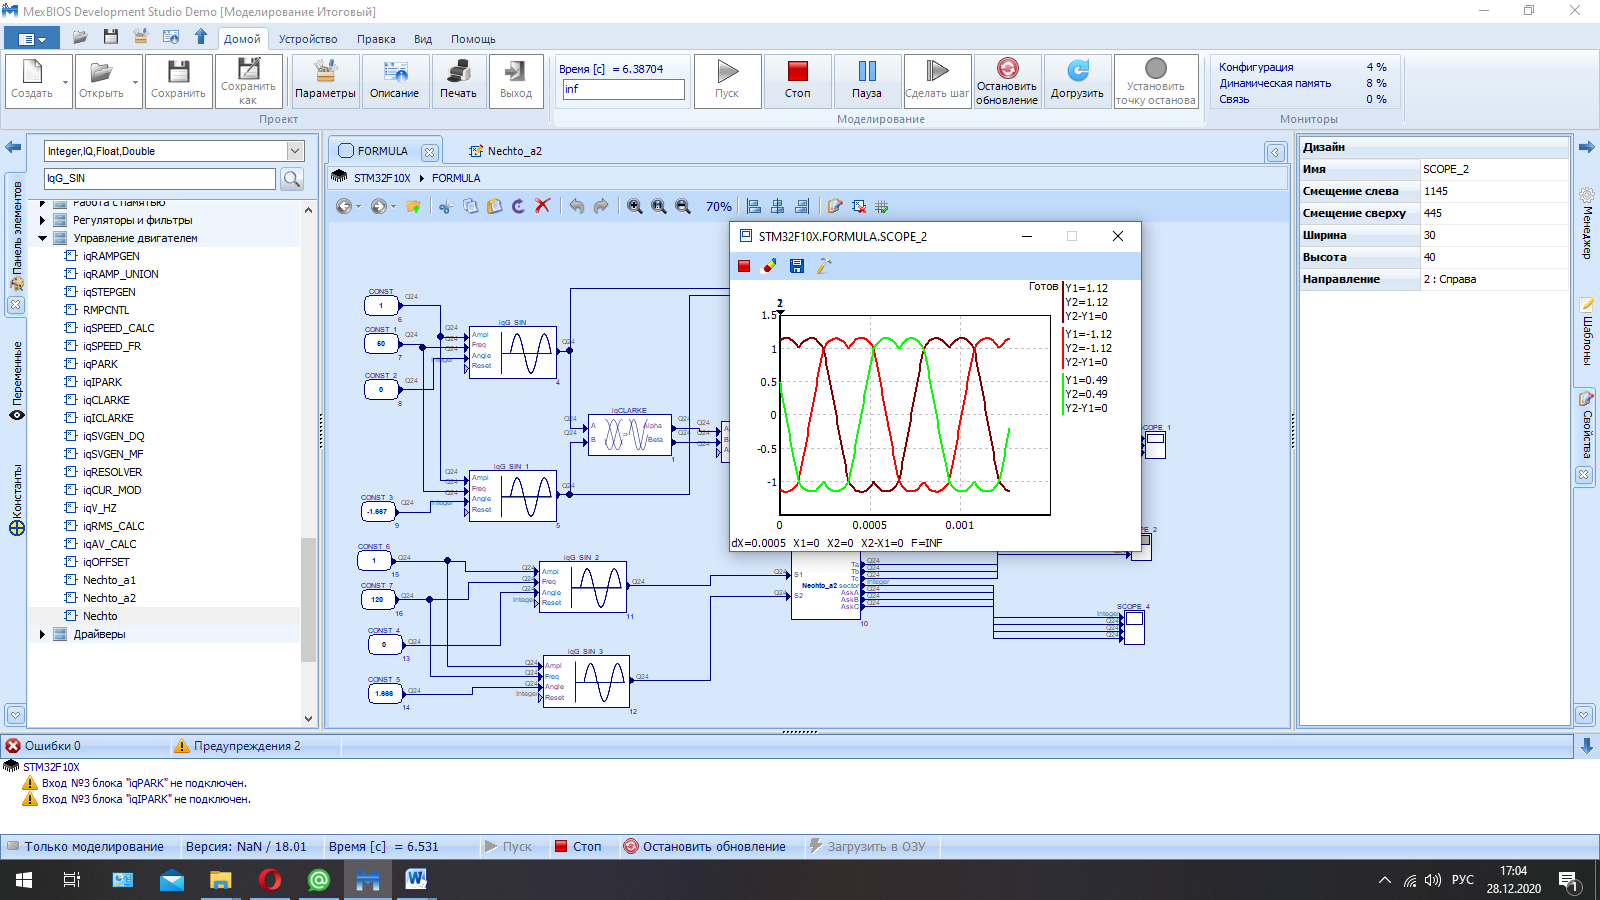
\includegraphics[width=1.0\linewidth]{custom_scope}
\caption{проверка алгоритма c использованием ковариантных и контравариантных координат для управления двигателем в среде MexBIOS}
\end{figure}

\newpage
\begin{figure}[ht!]
\centering
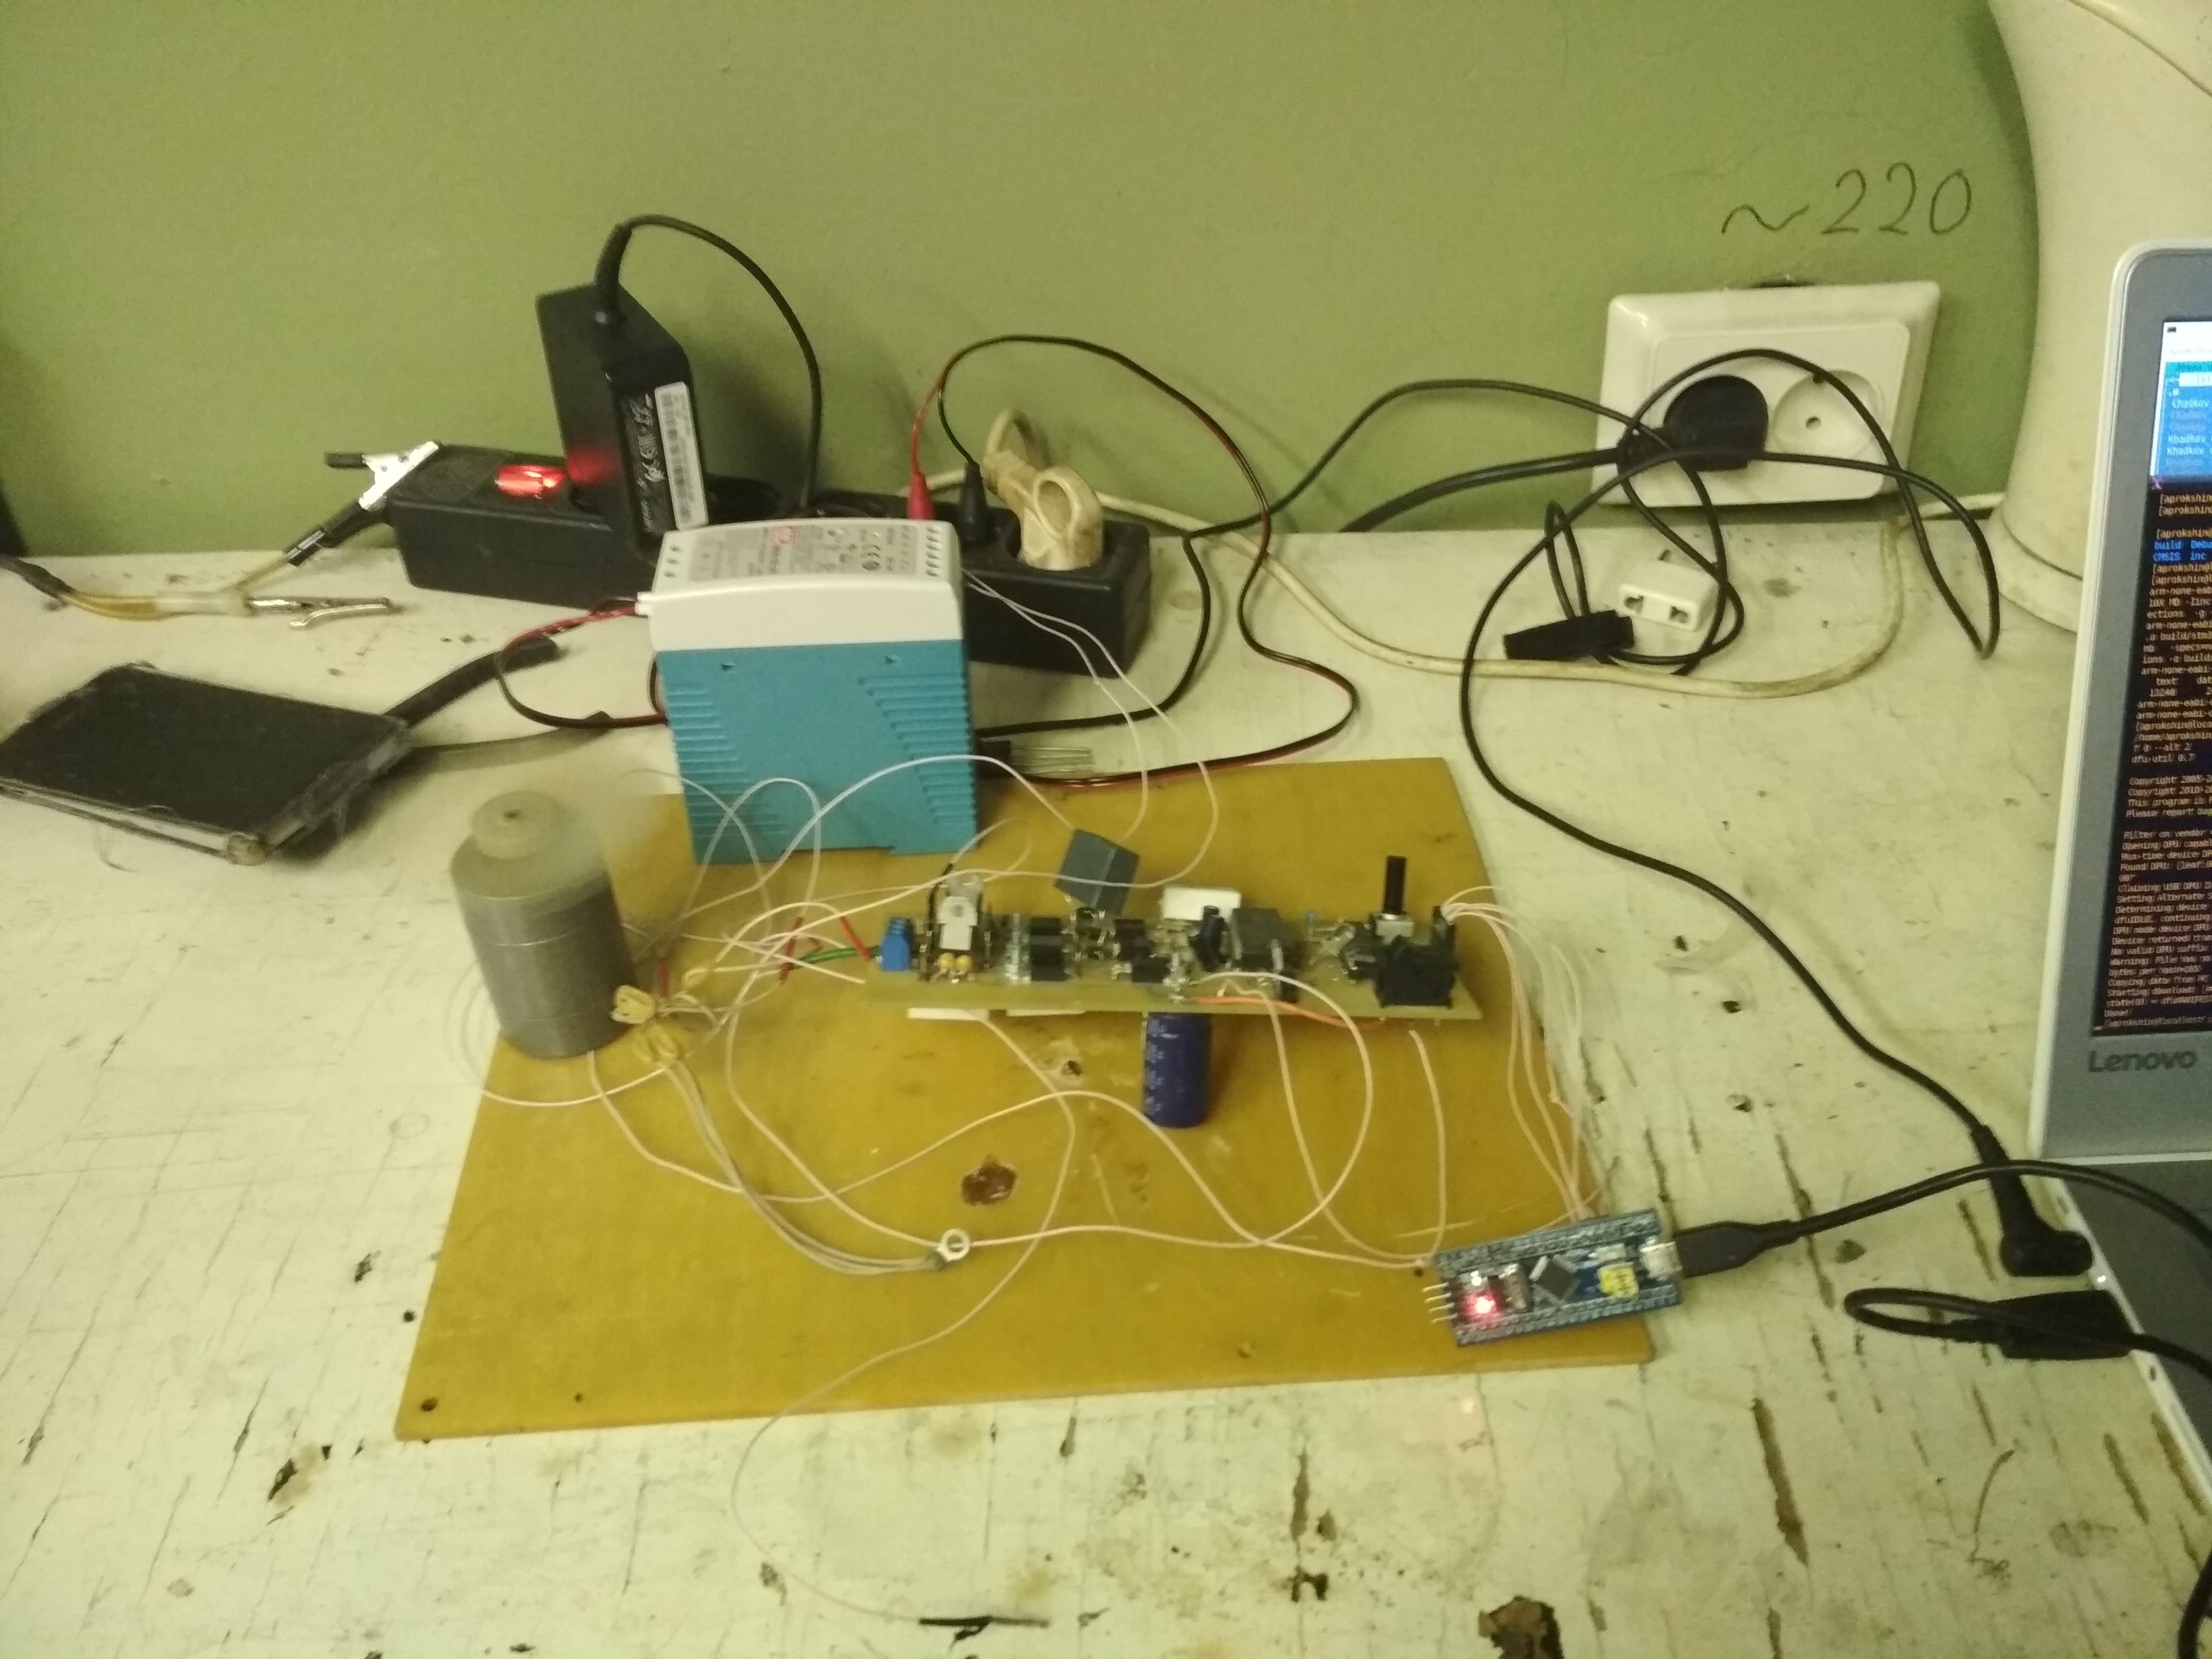
\includegraphics[width=0.9\linewidth]{IMG_20181222_105931}
\caption{результат работы программы на stm32f103c8t6 для кейса №1}
\end{figure}
\begin{figure}[ht!]
\centering
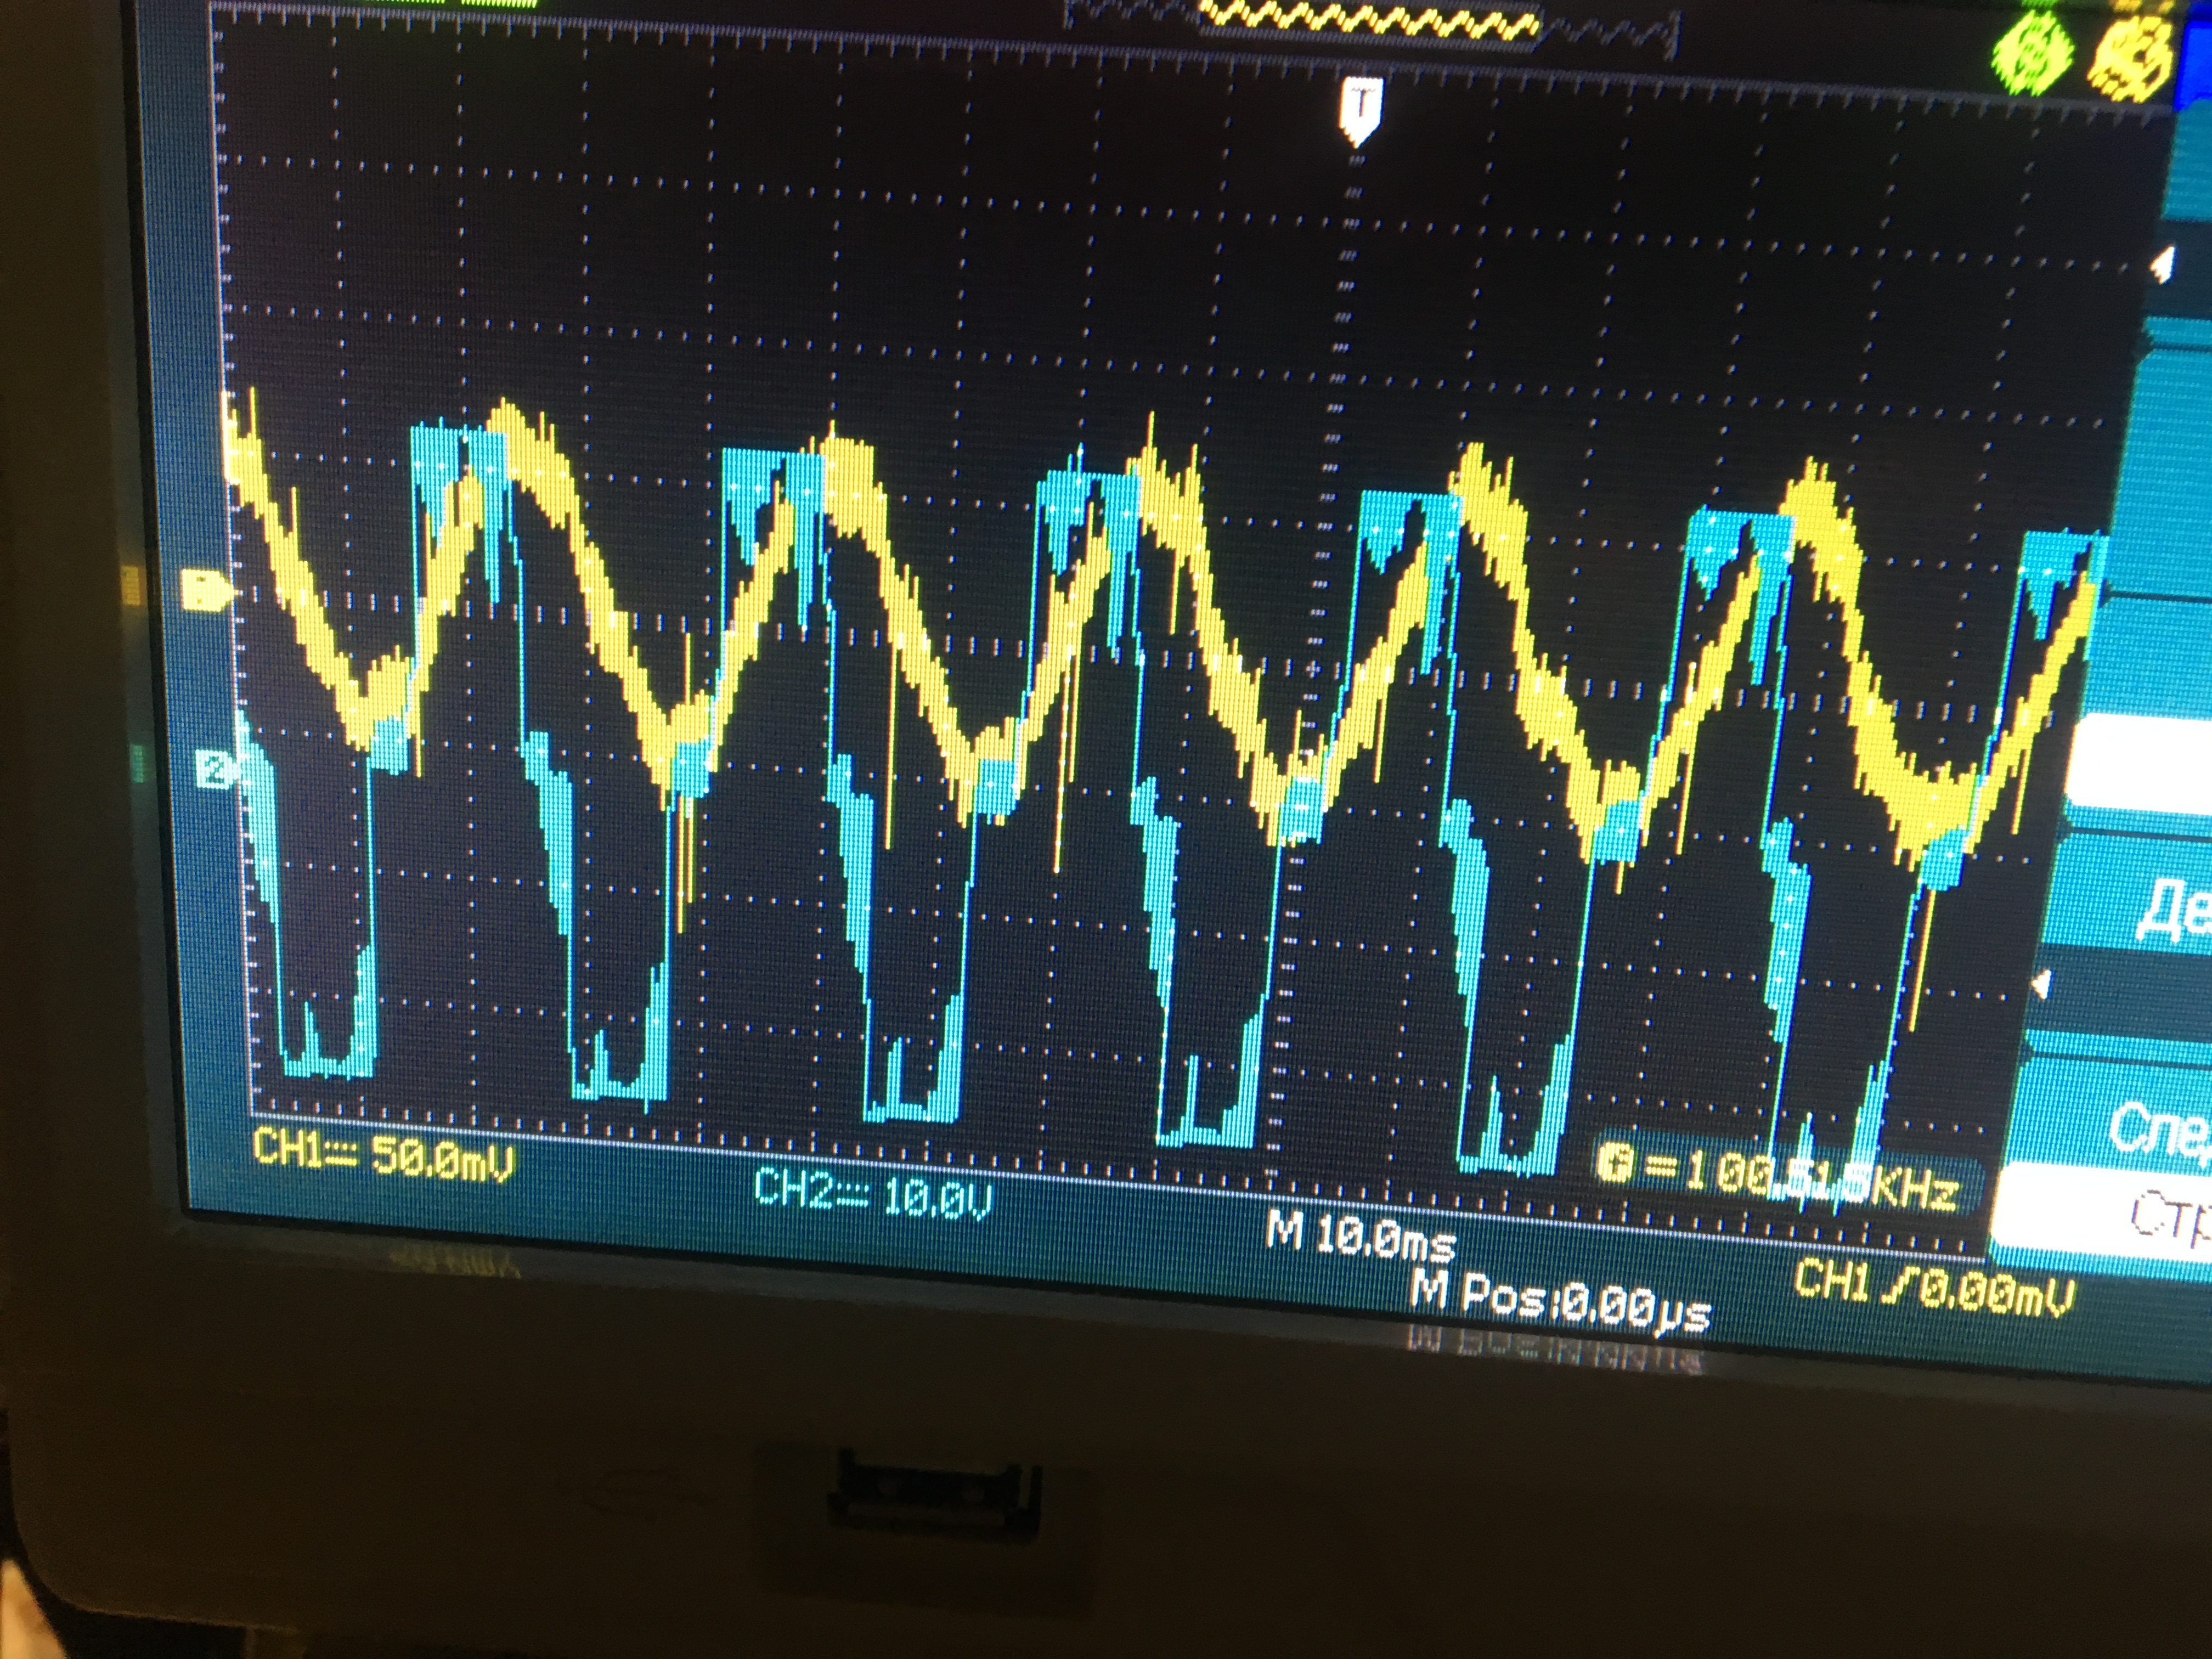
\includegraphics[width=0.9\linewidth]{4IMG_3171}
\caption{\color{yellow}{фазный ток} \color{black}{и} \color{blue}{линейное напряжение} \color{black}{на выходе инвертора}}
\end{figure}

\newpage
\section{Учебно-методическое и информационное обеспечение}
\begin{itemize}
\item Перечень основной учебной литературы
\begin{enumerate}
           \item \small{\footnotesize{
               Прокшин А.Н. и др.
              \href{https://scm.etu.ru/assets/files/2021/scm21/papers/113-115.pdf}
              {Измерение тока и напряжения в \colorbox{yellow}{косоугольных координатах} в трехфазной обобщенной электрической машине
               XXIV Международная конференция по мягким вычислениям и измерениям (SCM'2021)}}}
           \item \small{\footnotesize{
               Прокшин А.Н. и др.
               \href{https://etu.ru/assets/files/university/irvc/konferencii/2019/pps/sbornik-72-pps-2019.pdf}
                { Создание и апробирование \colorbox{yellow}{лабораторных работ по дисципли}-\colorbox{yellow}{нам «микроконтроллеры»} и «цифровая и микропроцессорная техника в управлении»
                  Сборник докладов 72 научно-технической конференции ППС, 2019г, с. 134-138}}}
           \item \small{\footnotesize{
               Прокшин А.Н. и др.
               \href{https://conf-ntores.etu.ru/assets/files/2021/cp/papers/331-332.pdf}
               {\colorbox{yellow}{Создание лабораторных работ} по дисциплине «Цифровая и микропроцессорная техника в управлении» с использованием российского программного обеспечения «MexBIOS Development Studio 6.21»}}}
           \item \small{\footnotesize{
               Прокшин А.Н. и др.
               \href{https://etu.ru/assets/files/university/irvc/konferencii/2018/pps-2018.pdf}
               {О системах координат для математического описания систем управления электропривода Сборник докладов 71-й научно-технической конференции ППС, СПб, 2018, с.172-175}}}
        \item \small{\footnotesize{ Соколовский Г.Г. Электроприводы переменного тока с частотным регулированием: Учебник для студ. высш.учеб.заведений.
                -- М. «Академия», 2007 - 272 с.}}
         \item \small{\footnotesize{Ю.Н. Калачев SimInTech: моделирование в электроприводе -- М.изд. ДМК, 2019 -- 95 с.}}
         \item \small{\footnotesize{С.Г.Герман-Галкин и др. Модельное проектирование электромеханических мехатронных модулей движения в среде SimInTech -- M.изд. ДМК, 2020 -- 494 с.}}

\end{enumerate}
\item Перечень дополнительной литературы
\begin{enumerate}
          \item \small{\footnotesize{А.А.Горев Переходные процессы синхронной машины -- М.,Л., Гос. энергетическое изд., 1950. -- 551 c.}}
          \item \small{\footnotesize{Программа для векторной широтно-импульсной модуляции для системы управления трехфазной электрической машиной с использованием \colorbox{yellow}{ковариантных и контра-}
                   \colorbox{yellow}{вариантных координат изображающего вектора}. Свидетельство о государственной регистрации программы для ЭВМ}}
          \item \small{\footnotesize{Программа для системы управления трехфазной электрической машиной c векторной широтно-импульсной модуляцией. Свидетельство о государственной регистрации программы для ЭВМ №2020662398 от 13 октября 2020}}
          \item \small{\footnotesize{\colorbox{yellow}{Веб интерфейс к ngspice} (NG-Spice web interface). Свидетельство о государственной регистрации программы для ЭВМ}}
\end{enumerate}
\item Учебно-методическое и информационное обеспечение
\begin{enumerate}
        \item \colorbox{yellow}{\href{overleaf.com}{overleaf} или \href{sharelatex.com}{sharelatex}}
         \item \colorbox{yellow}{\href{github.com}{github}, \href{gitlab.com}{gitlab}, \href{bitbucket.org}{bitbucket}}
         \item \colorbox{yellow}{\href{https://mechatronica-pro.com/ru}{MexBIOS}}
         \item \colorbox{yellow}{\href{https://simintech.ru/}{SimInTech}}
         \item \colorbox{yellow}{\href{https://www.mycompiler.io/new/c}{песочница С}}
         \item \colorbox{yellow}{\href{https://easyeda.com/}{easyEDA}}

\end{enumerate}
\end{itemize}
\end{document}
